\section{Validación Experimental} \label{sec:experimental_eval_fair}

\definecolor{Gray}{gray}{0.9}
\definecolor{Gray2}{gray}{0.95}
\newcolumntype{g}{>{\columncolor{Gray}}c}
\newcolumntype{h}{>{\columncolor{Gray2}}c}

Para evaluar la viabilidad de nuestro enfoque, hemos ampliado sobre el model checker {\Prism}~\cite{DBLP:conf/cav/KwiatkowskaN0S20,DBLP:conf/cav/KwiatkowskaNP11} con un operador para calcular las recompensas esperadas de los juegos estocásticos terminantes bajo fairness. El prototipo de esta herramienta también permite verificar si un juego se detiene bajo fairness.
%implementó una herramienta prototipo llamada \textsf{SynthFairy} (disponible en \cite{SynthFairy})
% y ejecútelo en dos conjuntos diferentes de ejemplos. %\footnote{Disponible en \cite{SynthFairy}}.
La herramienta toma como entrada un modelo que describe el juego en notación {\Prism} y devuelve como salida
la recompensa total esperada óptima para un estado inicial dado, así como la estrategia de controlador óptima sintetizada (bajo supuestos de fairness sobre el ambiente).
%Los modelos de entrada se especifican usando un lenguaje parecido a la notación {\Prism} \cite{DBLP:conf/cav/KwiatkowskaNP11}.
La evaluación experimental muestra que nuestro enfoque puede hacer frente a estudios de casos no triviales. Para calcular estos valores establecemos un error relativo de como máximo $\varepsilon = 10^{-6}$.


%We have considered variations of two examples:
%For the model presented in Sec.~\ref{sec:mot_example}, the expected total reward when $\verb"P"=0.1$ and $\verb"Q"=0$ is $5.55$. Moreover, 
%the non-trivial part of the synthesized strategy is illustrated with the black arrows in Fig.~\ref{fig:robot_game_grid}.
\paragraph{Roborta vs. la Luz fair.}
Consideramos tres variantes del caso de estudio: versión A (la luz no falla), versión B (la luz solo puede fallar cuando intenta dar una luz verde) y versión C (la luz puede fallar cuando intenta señalar cualquier tipo de luz).
Asumimos que, cuando Roborta falla, no puede moverse (esto es beneficioso para Roborta ya que puede recuperar la recompensa);
cuando falla la luz, el robot puede moverse libremente en cualquier dirección permitida.
La configuración de la matriz (restricciones de movimiento y recompensas) se genera aleatoriamente. Para cada configuración, la Tabla~\ref{table:resultsRobot} describe los resultados para tres escenarios diferentes generados a partir de semillas diferentes. La primera columna describe el tamaño de la matriz. La segunda columna indica la probabilidad de fallo del robot ($P$) y la luz ($Q$).
Las otras columnas describen el tamaño del modelo, la recompensa total esperada para la estrategia óptima y el número de iteraciones realizadas, respectivamente para tres configuraciones diferentes generadas aleatoriamente.
Para la configuración de matriz que se muestra en Sección~\ref{sec:mot_example_fair} con parámetros $P=0.1$ y $Q=0$, la herramienta derivó la estrategia óptima representada en la Figura~\ref{fig:robot_game_grid} e informa una recompensa total esperada de $5.55$.


%We explain Table~\ref{table:resultsRobot} with an example.  Take the case of the grid $A \mid {60{\times}8} \mid \text{seed } 1$, with the robot fault probability being $0.1$, the optimal expected total reward is $26.66$ and the number of decisions made by the robot when both players play optimally is $2$.  We consider a decision as a choice resolution introduced when the yellow light is on on a cell without movement restrictions or if the light is off. We use this number to give us an idea that resolutions are not trivial, and to hint a different resolution for closely related instances.
%Indeed, notice that for the case mentioned above, when the fault probability is set to $0.9$ (instead of $0.1$), the number of decisions changes to $0$. 
%This suggests that the strategy of the environment for lower fault probabilities was not worth it anymore, thereby it finds a better strategy. 

\begin{table}[tp]
  \centering\noindent%
  %\vspace{-0.5cm}
  %\vspace{-0.8cm}
  \scalebox{0.7}{
    \small
    \begin{tabular}{|c|c|c|c|c|c|g|h|c|g|h|c|}
      \hline
      \multirow{2}{*}{Versión} & \multicolumn{2}{c|}{Prob.Falla} & \multicolumn{3}{c|}{Tamaño (Estados/Transiciones)} & \multicolumn{3}{c|}{Rec.\ Total.\ Esp. Opt.} & \multicolumn{3}{c|}{Iteraciones}\\ \hhline{|~|-|-|-|-|-|-|-|-|-|-|-|}
      & $P$ & $Q$ &  \cellcolor{white}s.\ 1 & \cellcolor{white}s.\ 2 & \cellcolor{white}s.\ 3 & \cellcolor{white}\makebox[3.4em][c]{s.\ 1} & \cellcolor{white}\makebox[3.4em][c]{s.\ 2} & \cellcolor{white}\makebox[3.4em][c]{s.\ 3} & \cellcolor{white}\makebox[1.8em][c]{s.\ 1} & \cellcolor{white}\makebox[1.8em][c]{s.\ 2} & \cellcolor{white}\makebox[1.8em][c]{s.\ 3}  \\  
      \hline
       \multirow{2}{3em}{\centering $A$ \\ $60{\times}8$}
       & $0.1$ & $-$ & \multirow{2}{*}{\centering $\displaystyle \begin{array}{c} \text{st. }1448 \\ \text{tr. }3220 \end{array}$} & \multirow{2}{*}{\centering $\displaystyle \begin{array}{c} \text{st. }1418 \\ \text{tr. }3112 \end{array}$}  & \multirow{2}{*}{\centering $\displaystyle \begin{array}{c} \text{st. }1421 \\ \text{tr. }3132 \end{array}$}  & $26.66$ & $31.11$ & $27.77$ & $711$ & $681$ & $252$\\ \hhline{|~|-|-|~|~|~|-|-|-|-|-|-|}
       & $0.5$ & $-$ & & & & $48$ & $56$ & $50$ & $2253$ & $2225$ & $475$\\ \hline

       \multirow{2}{3em}{\centering $A$ \\ $120{\times}16$}
       & $0.1$ & $-$ & \multirow{2}{*}{\centering $\displaystyle \begin{array}{c} \text{st. }5686 \\ \text{tr. }12586 \end{array}$} & \multirow{2}{*}{\centering $\displaystyle \begin{array}{c} \text{st. }5716 \\ \text{tr. }12658 \end{array}$}  & \multirow{2}{*}{\centering $\displaystyle \begin{array}{c} \text{st. }5716 \\ \text{tr. }12722 \end{array}$}  & $62.22$ & $55.55$ & $48.88$ & $687$ & $700$ & $685$ \\ \hhline{|~|-|-|~|~|~|-|-|-|-|-|-|}
       & $0.5$ & $-$ & & & & $112$ & $100$ & $88$ & $2231$ & $2265$ & $2229$ \\ \hline

       \multirow{4}{3em}{\centering $B$ \\ $60{\times}8$}
       & \multirow{2}{*}{$0.1$} & $0.1$ & \multirow{4}{*}{\centering $\displaystyle \begin{array}{c} \text{st. }1928 \\ \text{tr. }5952 \end{array}$} & \multirow{4}{*}{\centering $\displaystyle \begin{array}{c} \text{st. }1888 \\ \text{tr. }5746 \end{array}$}  & \multirow{4}{*}{\centering $\displaystyle \begin{array}{c} \text{st. }1892 \\ \text{tr. }5785 \end{array}$}  & $42.6$ & $44.59$ & $42.23$ & $479$ & $335$ & $388$ \\ \hhline{|~|~|-|~|~|~|-|-|-|-|-|-|}
       & & $0.5$ & & & & $130.14$ & $127.7$ & $136.22$ & $772$ & $689$ & $824$ \\ \hhline{|~|-|-|~|~|~|-|-|-|-|-|-|}
       & \multirow{2}{*}{$0.5$} & $0.1$ & & & & $76.68$ & $80.26$ & $76.02$ & $873$ & $764$ & $909$ \\ \hhline{|~|~|-|~|~|~|-|-|-|-|-|-|}
       & & $0.5$ & & & & $234.26$ & $229.87$ & $245.21$ & $1263$ & $1139$ & $1341$ \\ \hline

       \multirow{4}{3em}{\centering $B$ \\ $120{\times}16$}
       & \multirow{2}{*}{$0.1$} & $0.1$ & \multirow{4}{*}{\centering $\displaystyle \begin{array}{c} \text{st. }7576 \\ \text{tr. }23266 \end{array}$} & \multirow{4}{*}{\centering $\displaystyle \begin{array}{c} \text{st. }7616 \\ \text{tr. }23400 \end{array}$}  & \multirow{4}{*}{\centering $\displaystyle \begin{array}{c} \text{st. }7616 \\ \text{tr. }23528 \end{array}$}  & $91.19$ & $87.27$ & $80.07$ & $538$ & $544$ & $616$ \\ \hhline{|~|~|-|~|~|~|-|-|-|-|-|-|}
       & & $0.5$ & & & & $281.83$ & $281.48$ & $265.33$ & $1076$ & $1118$ & $1252$\\ \hhline{|~|-|-|~|~|~|-|-|-|-|-|-|}
       & \multirow{2}{*}{$0.5$} & $0.1$ & & & & $164.15$ & $157.1$ & $144.13$ & $1147$ & $1223$ & $1373$ \\ \hhline{|~|~|-|~|~|~|-|-|-|-|-|-|}
       & & $0.5$ & & & & $507.30$ & $506.67$ & $477.6$ & $1850$ & $1865$ & $2088$ \\ \hline

       \multirow{4}{3em}{\centering $C$ \\ $60{\times}8$}
       & \multirow{2}{*}{$0.1$} & $0.1$ & \multirow{4}{*}{\centering $\displaystyle \begin{array}{c} \text{st. }1928 \\ \text{tr. }6432 \end{array}$} & \multirow{4}{*}{\centering $\displaystyle \begin{array}{c} \text{st. }1888 \\ \text{tr. }6216 \end{array}$}  & \multirow{4}{*}{\centering $\displaystyle \begin{array}{c} \text{st. }1892 \\ \text{tr. }6256 \end{array}$}  & $46.32$ & $47.07$ & $44.87$ & $379$ & $336$ & $390$ \\ \hhline{|~|~|-|~|~|~|-|-|-|-|-|-|}
       & & $0.5$ & & & & $143.35$ & $146.41$ & $153.98$ & $742$ & $658$ & $774$ \\ \hhline{|~|-|-|~|~|~|-|-|-|-|-|-|}
       & \multirow{2}{*}{$0.5$} & $0.1$ & & & & $83.37$ & $84.73$ & $80.77$ & $879$ & $769$ & $914$ \\ \hhline{|~|~|-|~|~|~|-|-|-|-|-|-|}
       & & $0.5$ & & & & $258.04$ & $263.53$ & $277.17$ & $1202$ & $1076$ & $1246$ \\ \hline

       \multirow{4}{3em}{\centering $C$ \\ $120{\times}16$}
       & \multirow{2}{*}{$0.1$} & $0.1$ & \multirow{4}{*}{\centering $\displaystyle \begin{array}{c} \text{st. }7576 \\ \text{tr. }25156 \end{array}$} & \multirow{4}{*}{\centering $\displaystyle \begin{array}{c} \text{st. }7616 \\ \text{tr. }25300 \end{array}$}  & \multirow{4}{*}{\centering $\displaystyle \begin{array}{c} \text{st. }7616 \\ \text{tr. }25428 \end{array}$}  & $98.25$ & $93.74$ & $88.33$ & $533$ & $544$ & $606$ \\ \hhline{|~|~|-|~|~|~|-|-|-|-|-|-|}
       & & $0.5$ & & & & $321.18$ & $317.61$ & $311.62$ & $1002$ & $1068$ & $1188$ \\ \hhline{|~|-|-|~|~|~|-|-|-|-|-|-|}
       & \multirow{2}{*}{$0.5$} & $0.1$ & & & & $176.85$ & $168.73$ & $158.99$ & $1147$ & $1227$ & $1365$\\ \hhline{|~|~|-|~|~|~|-|-|-|-|-|-|}
       & & $0.5$ & & & & $578.13$ & $571.71$ & $560.92$ & $1700$ & $1760$ & $1956$ \\ 

      \hline
    \end{tabular}
  }
  \caption{Resultados del juego Roborta vs. la Luz fair.}
  \label{table:resultsRobot}
  %\vspace{-0.8cm}
\end{table}


% Figure follows ------------------
\begin{figure}
%\vspace{-10mm}
%\vspace{-11mm}
%\fontsize{6.6}{6.6}\selectfont\ttfamily
\centering
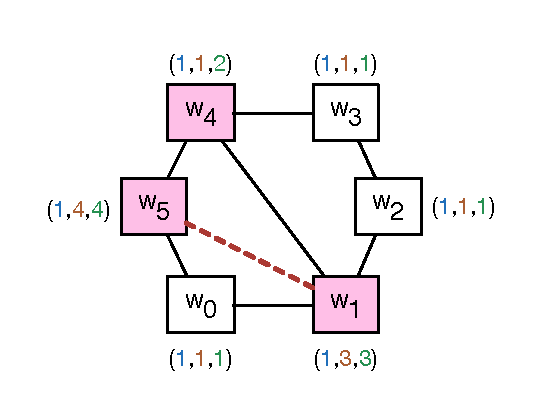
\includegraphics[scale=0.80]{Figs/uav.eps}
%\vspace{-10mm}
\caption{Red UAV para misiones ISR} \label{fig:uav_game_map}
%\caption{A robot game on a $4 \times 4$ grid starting on location (0,0). Each location has an assigned positive reward. The sideway movement restrictions are depicted as white arrows on the bottom-right of each location. The best strategy for the robot when the light is yellow is shown in black arrows on the top-right of the locations without movement restrictions. The path taken by the robot to achieve the goal is highlighted in yellow} \label{fig:robot_game_grid}
\end{figure}
%
\paragraph{UAV autónomo vs. Operador humano.} Adaptamos el caso de estudio analizado en \cite{DBLP:conf/iccps/FengWHT15}. Se utiliza un vehículo aéreo no tripulado (UAV) controlado a distancia para realizar misiones de inteligencia, vigilancia y reconocimiento (ISR) en una red de carreteras. El UAV realiza funciones de pilotaje de forma autónoma (seleccionando una ruta para volar entre \emph{puntos de referencia}). El operador humano (entorno) controla el sensor a bordo para capturar imágenes en un punto de ruta, así como las funciones de pilotaje en ciertos puntos de ruta (llamados puntos de control). Tenga en cuenta que un operador puede tratar continuamente de obtener una mejor imagen haciendo que el UAV merodee alrededor de un determinado punto de referencia, lo que puede conducir a un comportamiento infair.
%Asignamos recompensas a una captura exitosa de un waypoint no visitado.
Cada captura exitosa de un punto de referencia no visitado otorga una recompensa.

%
La Figura~\ref{fig:uav_game_map} muestra un ejemplo de red de carreteras que consta de seis puntos de referencia de vigilancia etiquetados $w_0,w_2,...,w_5$, los bordes representan rutas de conexión, una línea discontinua roja significa que la ruta es lo suficientemente peligrosa como para hacer que el UAV deje de funcionar con una probabilidad de $1$, mientras que en cualquier otro camino, esta probabilidad es de $S$. Los puntos de control se representan como nodos rosas, en los que el operador aún puede delegar la tarea de pilotaje al UAV con probabilidad $D$. Cada nodo está anotado con tres posibles recompensas. Por ejemplo, para $S=0.3$ y $D=0.5$ y los valores de recompensa más a la izquierda en cada terna, la estrategia sintetizada para el UAV intenta seguir el circuito óptimo $w_0,w_1,w_2,w_3,w_4,w_5$. Mientras que para los valores de recompensa del medio y más a la derecha, los circuitos óptimos a seguir son $w_0,w_5,w_0,w_1,w_2,w_3,w_4$ y $w_0,w_5,w_4,w_1,w_2,w_3$, respectivamente. 
La Tabla~\ref{table:resultsUAV} muestra los resultados obtenidos para este juego para varias redes de carreteras generadas aleatoriamente. La primera columna describe el número de puntos de referencia utilizados. La segunda columna indica la probabilidad de delegación ($D$) y la probabilidad de que el UAV deje de funcionar ($S$).
Las otras columnas muestran el tamaño del modelo, la recompensa total esperada para la estrategia óptima y el número de iteraciones realizadas, respectivamente, para tres configuraciones diferentes de mapas de ruta generadas aleatoriamente.

Las tablas~\ref{table:resultsRobot} y~\ref{table:resultsUAV} no informan el tiempo necesario para calcular los resultados, pero en todos los casos la salida se calculó en menos de 400 segundos. Todos los experimentos se realizaron en un MacBook Air con Intel Core i5 a 1,3 GHz y 4 GB de RAM. Tanto la herramienta como los casos de estudio se encuentran disponibles en un repositorio github~\cite{FairPrism}.

\begin{table}[h]
  \centering\noindent%
  %\vspace{-0.5cm}
  %\vspace{-0.8cm}
  \scalebox{0.7}{
    \small
    \begin{tabular}{|c|c|c|c|c|c|g|h|c|g|h|c|}
      \hline
      \multirow{2}{*}{Versión} & \multicolumn{2}{c|}{Prob.} & \multicolumn{3}{c|}{Tamaño(Estados/Transiciones)} & \multicolumn{3}{c|}{Rec.\ Total.\ Esp. Opt.} & \multicolumn{3}{c|}{Iteraciones} \\ \hhline{|~|-|-|-|-|-|-|-|-|-|-|-|}
      & $D$ & $S$ &  \cellcolor{white}s.\ 1 & \cellcolor{white}s.\ 2 & \cellcolor{white}s.\ 3 & \cellcolor{white}\makebox[3.4em][c]{s.\ 1} & \cellcolor{white}\makebox[3.4em][c]{s.\ 2} & \cellcolor{white}\makebox[3.4em][c]{s.\ 3} & \cellcolor{white}\makebox[1.8em][c]{s.\ 1} & \cellcolor{white}\makebox[1.8em][c]{s.\ 2} & \cellcolor{white}\makebox[1.8em][c]{s.\ 3} \\  
      \hline
       \multirow{4}{3em}{\centering UAV \\ $6w.$}
       & \multirow{2}{*}{$0.1$} & $0.05$ & \multirow{4}{*}{\centering $\displaystyle \begin{array}{c} \text{st. }213 \\ \text{tr. }504 \end{array}$} & \multirow{4}{*}{\centering $\displaystyle \begin{array}{c} \text{st. }508 \\ \text{tr. }1368 \end{array}$} & \multirow{4}{*}{\centering $\displaystyle \begin{array}{c} \text{st. }136 \\ \text{tr. }312 \end{array}$} & $16.72$ & $12.47$ & $13.14$ & $142$ & $248$ & $22$ \\ \hhline{|~|~|-|~|~|~|-|-|-|-|-|-|}
       & & $0.1$ & & & & $15.73$ & $11.15$ & $12.63$ & $73$ & $188$ & $22$ \\ \hhline{|~|-|-|~|~|~|-|-|-|-|-|-|}
       & \multirow{2}{*}{$0.5$} & $0.05$ & & & & $20.49$ & $12.77$ & $17.05$ & $103$ & $133$ & $22$ \\ \hhline{|~|~|-|~|~|~|-|-|-|-|-|-|}
       & & $0.1$ & & & & $18.87$ & $11.67$ & $15.95$ & $55$ & $70$ & $22$ \\ \hline

       \multirow{4}{3em}{\centering UAV \\ $8w.$}
       & \multirow{2}{*}{$0.1$} & $0.05$ & \multirow{4}{*}{\centering $\displaystyle \begin{array}{c} \text{st. }2177 \\ \text{tr. }5959 \end{array}$} & \multirow{4}{*}{\centering $\displaystyle \begin{array}{c} \text{st. }3591 \\ \text{tr. }9991 \end{array}$} & \multirow{4}{*}{\centering $\displaystyle \begin{array}{c} \text{st. }1426 \\ \text{tr. }3604 \end{array}$} & $17.88$ & $40.59$ & $24.6$ & $407$ & $332$ & $779$ \\ \hhline{|~|~|-|~|~|~|-|-|-|-|-|-|}
       & & $0.1$ & & & & $17.11$ & $34.3$ & $21.48$ & $280$ & $233$ & $437$ \\ \hhline{|~|-|-|~|~|~|-|-|-|-|-|-|}
       & \multirow{2}{*}{$0.5$} & $0.05$ & & & & $26$ & $42.21$ & $30.87$ & $128$ & $214$ & $257$ \\ \hhline{|~|~|-|~|~|~|-|-|-|-|-|-|}
       & & $0.1$ & & & & $23.44$ & $36.08$ & $24.72$ & $116$ & $113$ & $194$ \\ \hline 

       \multirow{4}{3em}{\centering UAV \\ $10w.$}
       & \multirow{2}{*}{$0.1$} & $0.05$ & \multirow{4}{*}{\centering $\displaystyle \begin{array}{c} \text{st. }6631 \\ \text{tr. }17306 \end{array}$} & \multirow{4}{*}{\centering $\displaystyle \begin{array}{c} \text{st. }5072 \\ \text{tr. }13052 \end{array}$} & \multirow{4}{*}{\centering $\displaystyle \begin{array}{c} \text{st. }8272 \\ \text{tr. }24376 \end{array}$} & $39.76$ & $28.7$ & $19.76$ & $256$ & $377$ & $356$ \\ \hhline{|~|~|-|~|~|~|-|-|-|-|-|-|} 
       & & $0.1$ & & & & $35.43$ & $23.36$ & $16.2$ & $136$ & $260$ & $154$ \\ \hhline{|~|-|-|~|~|~|-|-|-|-|-|-|}
       & \multirow{2}{*}{$0.5$} & $0.05$ & & & & $42.13$ & $30.77$ & $24.56$ & $250$ & $247$ & $292$ \\ \hhline{|~|~|-|~|~|~|-|-|-|-|-|-|}
       & & $0.1$ & & & & $37.11$ & $26.08$ & $19.27$ & $130$ & $134$ & $151$\\ \hline

      \hline
    \end{tabular}
  }
   \caption{Resultados del juego UAV vs. Operador.}
  \label{table:resultsUAV}
  %\vspace{-0.8cm}
\end{table}








































































